%!TEX root = ../dokumentation.tex


\chapter{Auswertung und Darstellung mit Matlab}\label{chap:auswertung_matlab}

Die Daten werden nach Beendigung eines Scans exportiert und auf einem seperaten PC ausgewertet. Die Auswertung und Darstellung erfolgt mit Matlab. Matlab bietet sich an, da große Datenmengen schnell ausgewertet und dargestellt werden können. Zudem sind bereits Kenntnisse zum Importieren und Darstellen von .csv Dateien vorhanden. 

Die .csv Datei enthält die Rohdaten. Die Rohdaten bestehen pro Datenwert aus der Entfernung vom Messpunkt bis zum Hindernis in Zentimetern. Zudem ist jedem Entfernungswert der Azimut und der Polarwinkel (Elevation) im Bezug zum jeweils gesetzten Nullpunkt zugeordnet. Die Messwerte sind fortlaufend nummeriert. 
Diese Werte müssen zuerst aus der .csv Datei in Matlab importiert werden. Anschließend erfolgt die Aufteilung des Datensatzen in die Vektoren Entfernung, Azimut und Elevation.
Die beiden Winkelwerte zusammen mit dem Entfernungswert stellen Kugelkoordinaten dar. Diese müssen zur Darstellung in Matlab in kartesische Korrdinaten umgewandelt werden. 



\section{Importieren und Zuordnung der Messwerte}

Im ersten Teil des Auswertungs- und Darstellungsprogramms wird die .csv-Datei als Gesamtes in Matlab importiert. Anschließend werden die einzelnen Spalten dementsprechenden Variablen zugeordnet, um die spätere Auswerung zu erleichtern.

Das Importieren der Daten erfolgt über die ''importdata'' Funktion von Matlab. Diese ermöglicht es, Datensätze aus einer seperaten Datei zu lesen. Das erste Argument der Funktion ist der relative Dateipfad zu der einzulesenden Datei. Dieser wird in Zeile 5 festgelegt. Das zweite Argument steht für das Trennzeichen, mit dem einzelne Elemente in Daten abgetrennt werden. Bei .csv-Dateien ist dies ein Semikolon. Der letzte Übergabeparameter gibt an, wie viele Kopfzeilen importiert werden sollen.

Die importierten Daten liegen anschließend als Struct in der Variable "data" vor. Dieses Struct enthält zum einen die Kopfzeile als Feld und zum anderen die Messwerte ohne Kopfzeile. Für die weitere Verwendung der Daten, werden nur die Messwerte benötigt. Diese werden mit Zeile 8 extrahiert. 

Anschließend werden in Zeile 10 bis 12 die einzelnen Spalten separiert und einer passenden Variablen zugeordnet. 

\begin{lstlisting}[caption={Importieren und Zuordnen von .csv Dateien},language={Matlab}, label={import_data}, numbers=left]
% Anwendung zur Darstellung einer 3D Punktewolke aus einem LIDAR System
clear all;

% Importieren und Zuordnen der Messwerte
file = 'Messwerte-05-02/Aufloesung-hoch.csv';

data = importdata(file,';',1); 
data = data.data;

distance = data(:,2);
azimut = data(:,3);
elevation = data(:,4)
\end{lstlisting}


\section{Umwandlung von Kugelkoordinaten zu kartesischen Koordinaten}

Die Messpunkte liegen hardwarebedingt als Kugelkoordinaten vor. Dies bedeutet, dass jeder Punkt aus dem Abstand r zum Zentrum O, dem Polarwinkel $\theta$ und dem Azimutwinkel $\varphi$ definiert wird.

Der Abstand r wird durch die Distanz des Punktes P von 0 bestimmt. Der Polarwinkel $\theta$ ist der Winkel zwischen Flächennormalen und dem Vektor OP. Das Gegenstück dazu ist die Höhe.  Der Polarwinkel reicht von 0 bis $\pi$. \\
Der Azimutwinkel ist der Winkel zwischen der x-Achse und der Projektion der Strecke OP auf die xy Ebene. Dieser Winkel reicht je nach Definition von  -$\pi$ bis $\pi$ oder von 0 bis 2$\pi$. Für das Lidar System wird die zweite Definition verwendet.

\begin{figure}[H]
	\centering
	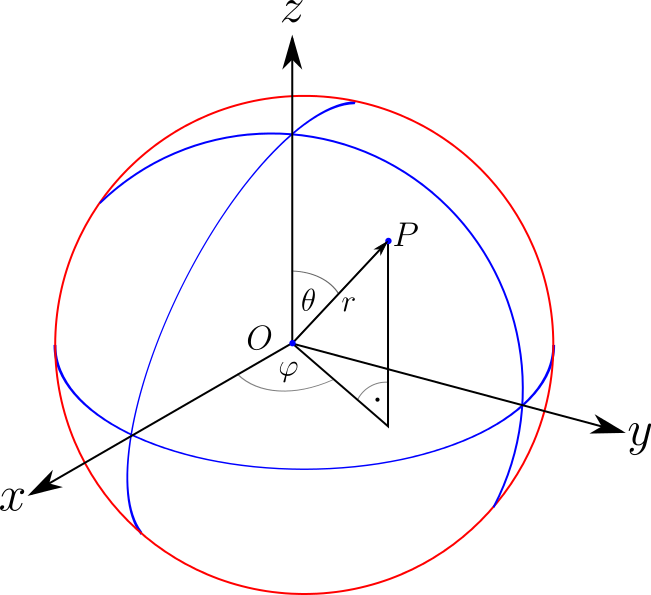
\includegraphics[width=0.75\textwidth]{images/Auswertung/Kugelkoordinaten}
	\caption{Kugelkoordinaten}
	\label{kugelkoordinaten}
\end{figure}



Da dass das Darstellen von Kugelkoordinaten in Matlab nicht ohne weiteres möglich ist, werden die Messwerte in kartesische Koordinaten umgerechnet.
Die Umrechnung erfolgt mit Formel \ref{umrechnung}:

\begin{equation}\formelentry{Umrechnung Kugelkoordinaten in kartesische Koordinaten}
\begin{split}
&x = r \cdot \cos(\theta) \cdot \cos(\varphi) \\
&y = r \cdot \cos(\theta) \cdot \sin(\varphi) \\
&z = r \cdot \sin(\theta)
\end{split}
\label{umrechnung}
\end{equation} 
\begin{flalign*}
&r = \text{Abstand des Punktes zum Zentrum} \left[m \right]&\\
&\theta = \text{Polarwinkel (Elevation)}\left[^{\circ} \right]&\\
&\varphi = \text{Azimutwinkel}\left[^{\circ} \right]&
\end{flalign*}

In Matlab wird jeder einzelne Punkt innerhalb eine For-Schleife mit der oben genannten Formel umgewandelt und die drei Koordinaten x,y und z für kartesische Koordinaten gespeichert. Als Endwert der Schleife wird die Zeilenanzahl des Datensatzes verwendet. Somit ist dieser Wert variabel und muss nicht für jeden Datensatz spezifisch angepasst werden.\\
Die Berechnung befindet sich zudem in einer If-Abfrage, welche dazu dient, offensichtliche Messfehler zu entfernen. Alle Koordinaten, bei denen die Entfernung höher als 10 Meter ist, werden gelöscht. Die 10 Meter wurden auf experimenteller Basis und aufgrund der Größe des vorher definierten Standardraums festgelegt. Beim Lidar TF Mini werden nicht messbare Entfernungen mit einer Entfernung von 34999 cm angegeben. Diese werden somit mit dieser Abfrage ebenfalls gefiltert.\\
Matlab rechnet bei trigonometrischer Funkionen mit dem Radiant. Die Winkel des Lidar Systems sind in Grad angegeben, weshalb sie innerhalb der Berechnung mit der Funktion deg2rad() in Radiant umgerechnet werden müssen.



\begin{lstlisting}[caption={Umwandlung von Kugelkoordinaten zu kartesischen Koordinaten},language={Matlab}, label={import_data}, numbers=left]
for i = 1:1:length(data)
	if(distance(i) < 1000)
		x(i) = -distance(i)*cos(deg2rad(elevation(i)))*cos(deg2rad(azimut(i)));
		y(i) = distance(i)*cos(deg2rad(elevation(i)))*sin(deg2rad(azimut(i)));
		z(i) = distance(i)*sin(deg2rad(elevation(i)));
	else
	end
end
\end{lstlisting}


\section{Darstellung der Messwerte}

Im letzten Teil des Programms werden die kartesischen Koordinatenpunkte in eine 3D-Darstellung umgewandelt. Zudem wird die Skalierung der Achsen festgelegt.


\begin{lstlisting}[caption={Darstellung der Messwerte},language={Matlab}, label={import_data}, numbers=left]
%plot3(x,y,z)			%Darstellung mit Linien
%plot3(x,y,z, '*')		%Darstellung mit Asteriskus 
plot3(x,y,z, '.')		%Darstellung mit kleinen Punkten
\end{lstlisting}

Die Darstellung der kartesischen Koordinaten erfolgt über die ''plot3()'' Funktion. Diese Funktion ermöglicht es, rotierbare, dreidimensionale Darstellungen anzufertigen. Die ersten drei Argumente der Funktion sind die Vektoren mit den jeweiligen Koordinaten.\\
Mit dem vierten Argument kann man die Darstellungsart der einzelnen Punkte festlegen. Anhand eines Datensatzes werden die drei verschiedene Möglichkeiten auf Vor- und Nachteile überprüft.

Übergibt man der Funktion keinen Parameter, werden die Punkte durch schmale Linien verbunden. Dadurch entsteht ein dreidimensionaler Raum, mit sehr feiner Darstellung. Konturen sind dabei sehr gut zu erkennen. Zudem kann man den Verlauf der Messwertaufnahme erkennen. \\
Nachteil dieser Darstellungsart ist, dass auch Messfehler verbunden werden, wodurch es zu fehlerhaften Darstellungen kommt. Dies ist beispielsweise in Abbildung \ref{linien} zu erkennen.


\begin{figure}[H]
	\centering
	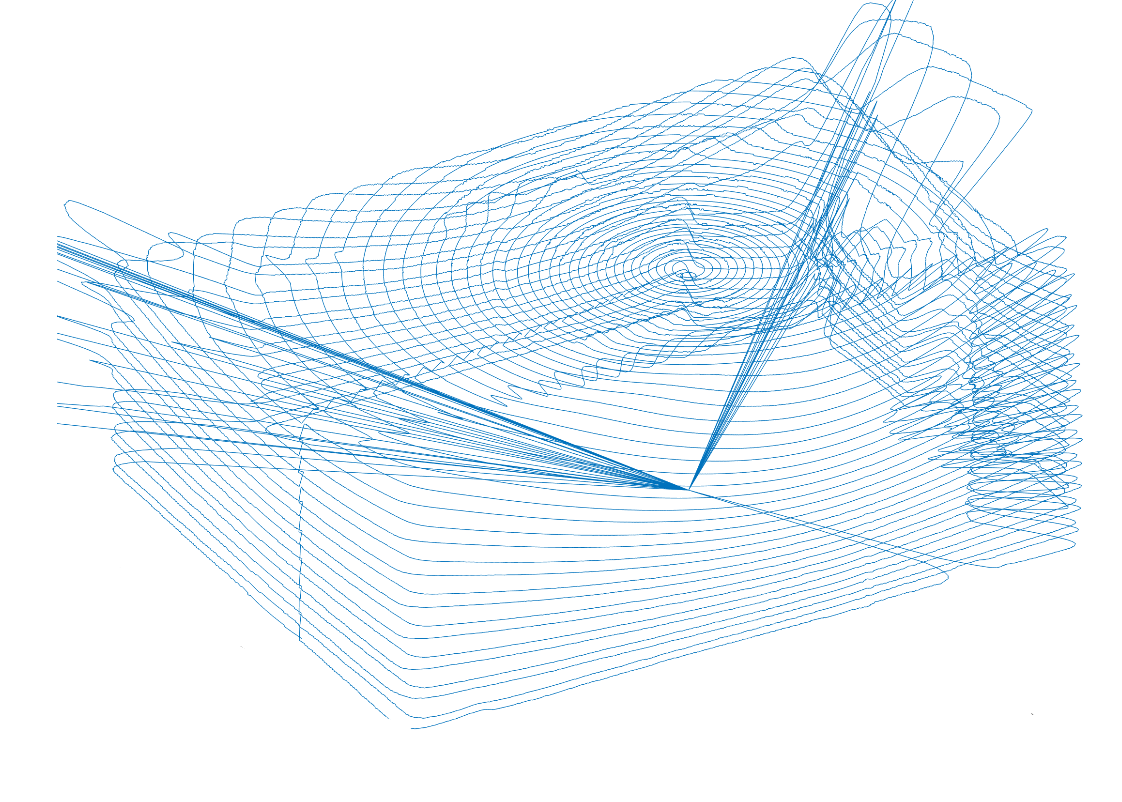
\includegraphics[width=0.7\textwidth]{images/Auswertung/Linien}
	\caption{Darstellung mit Linien}
	\label{linien}
\end{figure}

Einen weitere Möglichkeit der Darstellung sind Asterisken. Diese sind relativ zu den Linien sehr groß. Räume werden auch mit weniger Messpunkten erkennbar. Dadurch verschwimmen jedoch Aufnahmen mit höherer Auflösung und Details sind nicht mehr so gut erkennbar. 


\begin{figure}[H]
	\centering
	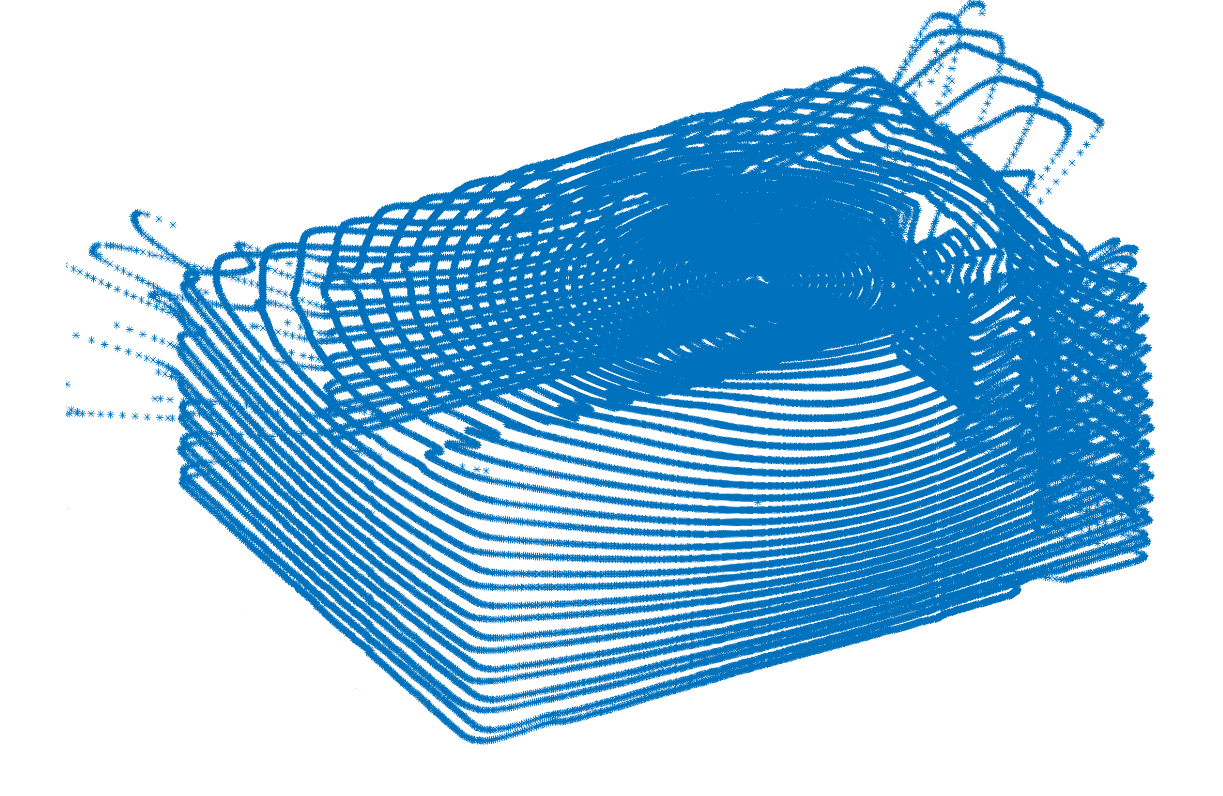
\includegraphics[width=0.7\textwidth]{images/Auswertung/Sternchen}
	\caption{Darstellung mit Asterisken}
	\label{asterisken}
\end{figure}

Die letzte Möglichkeit ist die Darstellung mit kleinen Koordinatenpunkten. Räume können bis ins sehr kleine Detail dargestellt werden und man hat trotz vieler Messpunkte und hoher Auflösung keine Stellen mit überladener Punkteanzahl. 



\begin{figure}[H]
	\centering
	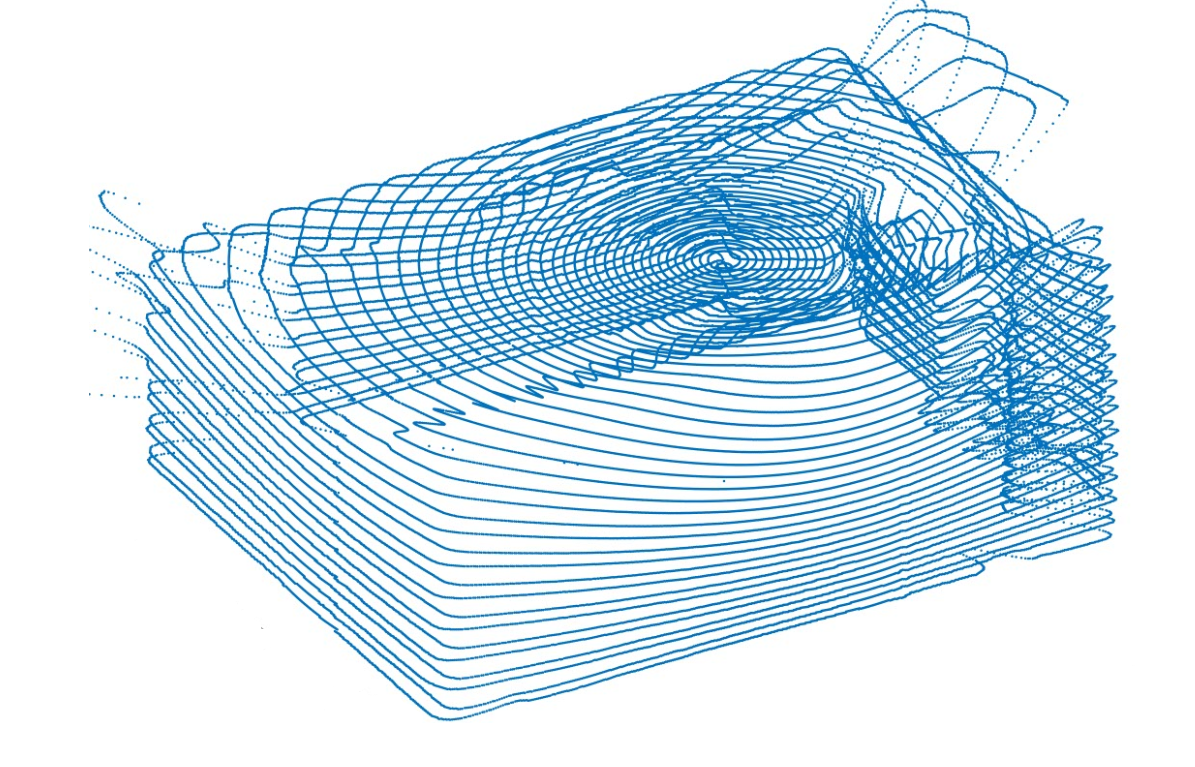
\includegraphics[width=0.7\textwidth]{images/Auswertung/Punkte}
	\caption{Darstellung mit Punkten}
	\label{punkte}
\end{figure}

Aufgrund der genannten Vor- und Nachteile wird in den meisten Fällen die Darstellung mit Punkten bevorzugt.  

Matlab skaliert die Achsen der Darstellung automatisch, weshalb teilweise schlecht auswertbare Bilder entstehen. Diese sind nur mit manueller Nachbearbeitung passend einstellbar. Um diese zusätzliche Arbeit zu automatisieren und die Darstellung einheitlich zu realisieren, werden die Achsen manuell mit der Funktion ''axis'' skaliert. Die ersten beiden Werte geben die Skala der x-Achse in Zentimetern an. Der zweite und dritte den Wert der y-Achse. Die letzten beiden Werte den Bereich der z-Achse.
Mit der Funktion ''pbaspect'' wird zudem die relative Größe der Achse in der späteren Darstellung festgelegt, um Verzerrungen zu vermeiden. 

\begin{lstlisting}[caption={Skalieren der Achsen},language={Matlab}, label={import_data}, numbers=left]
axis([-400 400 -400 400 0 240])
pbaspect([1 1 0.3])
\end{lstlisting}




